\icode{E-MI-SI-L2-261106-003}
一物体置于倾角为\(\theta\)的固定斜面上，物体与斜面间的动摩擦因数为\(\mu\)，先用平行于斜面的推力\(F_1\)作用于物体上，恰好能使该物体沿斜面匀速上滑，若改用水平推力\(F_2\)作用于该物体上，也恰好能使该物体沿斜面匀速上滑，则两次力之比\(\sfrac{F_1}{F_2}\)为\paren[]

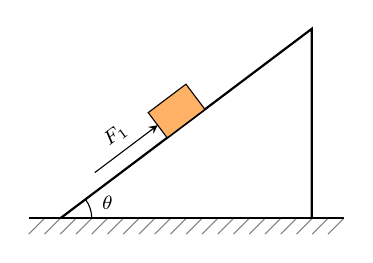
\begin{tikzpicture}[>=stealth,font=\scriptsize]
	\begin{scope}[rotate=37]
		\draw[thick] (0,0)--(4,0)--++(-127:2.4);
		\draw[fill=orange!60] (1.7,0) rectangle(2.3,.4);
		\draw[->] (.7,.2)--node[above,rotate=37]{\(F_1\)}(1.7,.2);
	\end{scope}
	\foreach \x in {-.4,-.2,...,3.4}
		\draw[gray] (\x,-.2)--++(.2,.2);
	\draw[thick] (-.4,0)--(3.6,0);
	\draw (.4,0) arc(0:37:.4);
	\node at(.6,.2){\(\theta\)};
\end{tikzpicture}
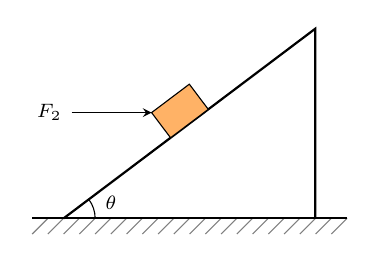
\begin{tikzpicture}[>=stealth,font=\scriptsize]
	\begin{scope}[rotate=37]
		\coordinate (O) at(1.7,.4);
		\draw[thick] (0,0)--(4,0)--++(-127:2.4);
		\draw[fill=orange!60] (1.7,0) rectangle(2.3,.4);
	\end{scope}
	\draw[->] (O-|.1,.3)node[left]{\(F_2\)}--(O);
	\foreach \x in {-.4,-.2,...,3.4}
		\draw[gray] (\x,-.2)--++(.2,.2);
	\draw[thick] (-.4,0)--(3.6,0);
	\draw (.4,0) arc(0:37:.4);
	\node at(.6,.2){\(\theta\)};
\end{tikzpicture}
\begin{choices}
	\item\(1 +\mu\tan\theta\)
	\item\(1 -\mu\tan\theta\)
	\item\(\cos\theta -\mu\sin\theta\)
	\item\(\cos\theta +\mu\sin\theta\)
\end{choices}
\begin{answer}
	C\qquad 提示：
\end{answer}